\section{Chemical Thermodynamics}
\subsection{Basic Concepts of Thermodynamics}
\begin{definition}[Thermodynamic System]
A thermodynamic system is a specific portion of matter selected for experimental or theoretical investigation. Everything outside the system is defined as its surroundings, and the universe is the sum of the system and its surroundings.
\end{definition}

Based on the exchange of matter and energy between the system and its surroundings, systems are classified into three categories:
\begin{enumerate}
    \item Open system: Exchanges both matter and energy with its surroundings;
    \item Closed system: Exchanges energy but not matter with its surroundings;
    \item Isolated system: Exchanges neither matter nor energy with its surroundings.
\end{enumerate}

A system is said to be in a definite state if all macroscopic physical properties describing it have uniquely determined values. A state function is a physical quantity whose change depends only on the initial and final states of the system, independent of the path taken for the change (e.g, volume $V$, temperature $T$, pressure $p$).

An extensive property is a state function that is additive for subsystems (e.g, volume $V$, amount of substance $n$, internal energy $U$). An intensive property is a state function that is non-additive and independent of the size of the system, typically the ratio of two extensive properties (e.g, pressure $p$, temperature $T$, density $\rho$).

A path function is a non-state function whose change depends on the specific path of the system's state transformation.

Having defined the system of interest, we can analyze its interactions with the surroundings from an energy perspective, analogous to analytical mechanics. The total energy of a system or its surroundings is called thermodynamic energy ($U$), also known as internal energy, whose absolute magnitude cannot be experimentally determined.

When two systems are in thermal contact, if there is no net energy transfer between them, the two systems are said to be in thermal equilibrium.

\begin{proposition}[Zeroth Law of Thermodynamics]
If two systems are each in thermal equilibrium with a third system, then the two systems are in thermal equilibrium with each other. In other words, thermal equilibrium defines an equivalence relation.
\end{proposition}

Since thermal equilibrium is an equivalence relation, we can assign a unique numerical value to each equivalence class, which we call temperature ($T$).

Based on temperature, interactions between the system and its surroundings are divided into two categories: one caused by a temperature difference, called heat ($Q$), and all other interactions are classified as work ($W$). Clearly, neither heat nor work is a state function.

An adiabatic process is defined as a process that permits work but no heat exchange between the system and its surroundings.

\begin{proposition}[First Law of Thermodynamics]
The change in internal energy of a closed system is equal to the sum of the work done on the system by the surroundings and the heat absorbed by the system. The core formula is:
$$\Delta U = U_f - U_i = W + Q$$
Its differential form is: (Note: $\mathrm{d}$ is used exclusively for state functions, while $\delta$ denotes an infinitesimal path-dependent quantity)
$$\mathrm{d}U = \delta W + \delta Q$$
where $\Delta U$ is the change in internal energy, $U_f$ and $U_i$ are the internal energy of the system in the final and initial states, respectively. $W$ is work, and $Q$ is heat. By sign convention, $W$ and $Q$ are positive when the system gains energy, and negative when the system loses energy.
\end{proposition}

For the universe, there are no surroundings, thus:
$$W=Q=0$$
meaning $U$ is constant. In other words, the total energy of the universe is conserved.

Next, we examine work and heat separately.

The most important type of work is expansion work ($W_e$), also called pressure-volume work, defined as the work done by the system against an external pressure due to a change in volume (or work done on the system by the surroundings). It follows the fundamental definition of work in mechanics: $\delta W=F \mathrm{d}r$. Noting the relationships between force and pressure, and between volume and displacement:
$$F = - p S, \quad \mathrm{d}V = S \mathrm{d}r$$
we derive:

\begin{proposition}[Expansion Work]
$$\delta W_e = -p_{ex}\mathrm{d}V, \quad W_e = \int_{V_1}^{V_2} -p_{ex}\mathrm{d}V$$
where $p_{ex}$ is the external pressure, and $\mathrm{d}V$ is the infinitesimal change in the system's volume. For an ideal gas, the expansion work for typical reversible processes is:
\begin{enumerate}
    \item Isobaric process ($p_{ex}=\text{constant}$): $W_e = -p(V_2 - V_1)$;
    \item Isothermal process ($T=\text{constant}$): $W_e = - \nu RT\ln\frac{V_2}{V_1}$;
    \item Isochoric process ($V=\text{constant}$): $W_e = 0$.
\end{enumerate}
\end{proposition}

All other forms of work are referred to as non-expansion work ($W_f$), which will be studied in later chapters. In this chapter, we assume no non-expansion work is present.

We first consider the isochoric state. In this case, $W = W_e + W_f = 0$. Combining with the First Law of Thermodynamics, $\Delta U = Q + W = Q$. We use the notation $Q_V$ to denote heat transfer at constant volume:

\begin{definition}[Isochoric (Reaction) Heat]
For a closed system with only expansion work ($W_f=0$), the heat absorbed or released by the system at constant volume ($Q_V$) is called isochoric heat. Its magnitude is equal to the change in the system's internal energy: $Q_V = \Delta U$.
\end{definition}

For an isobaric process, from our calculation of expansion work, we have $\Delta U = U_f - U_i = W + Q = - p_{ex} (V_f - V_i )$. Rearranging gives:
$$Q =(U_f + p_{ex} V_f ) - (U_i + p_{ex} V_i)$$
We observe that the quantity $U + pV$ characterizes heat transfer at constant pressure, so we define:

\begin{definition}[Enthalpy (Isobaric (Reaction) Heat)]
Enthalpy ($H$) is a state function defined as $H = U + pV$, whose state function property is described by Hess's Law. Clearly, its absolute magnitude cannot be experimentally determined.

For a closed system with only expansion work ($W_f=0$), the heat absorbed or released by the system at constant pressure ($Q_p$) is called isobaric heat. Its magnitude is equal to the change in the system's enthalpy: $Q_p = \Delta H$.
\end{definition}

\begin{proposition}[Relationship Between Enthalpy Change and Internal Energy Change]
For reactions involving gaseous species, the relationship between the enthalpy change and internal energy change is:
$$\Delta H = \Delta U + \Delta \nu_g RT$$
where $\Delta \nu_g = \sum \nu(\text{gaseous products}) - \sum \nu(\text{gaseous reactants})$ is the change in the moles of gaseous substances during the reaction.
\end{proposition}

Most chemical reaction systems operate under constant pressure, so we focus primarily on enthalpy. Since the absolute magnitude of enthalpy cannot be measured, we define a reference standard:

\begin{definition}[Standard Molar Enthalpy of Formation, Combustion, and Bond Enthalpy]
\begin{enumerate}
    \item Standard molar enthalpy of formation ($\Delta_f H_m^\circ$): The enthalpy change when 1 mole of a pure substance is formed from its most stable elemental forms in the standard state at a specified temperature (typically 298.15 K).
    \item Standard molar enthalpy of combustion ($\Delta_c H_m^\circ$): The enthalpy change when 1 mole of a pure substance undergoes complete combustion to form stable oxides in the standard state at a specified temperature.
    \item Bond enthalpy (bond dissociation energy, $BDE$): The enthalpy change when 1 mole of a specific chemical bond is broken in the gas phase at a specified temperature.
\end{enumerate}
\end{definition}

From the definition, enthalpy is a function of temperature due to the contribution from heat capacity changes ($\int C_p \,\mathrm{d}T$). This is beyond the scope of general chemistry and will not be discussed in detail here.

In these equations, we use a set of standard subscripts and superscripts: the subscript of $\Delta$ describes the type of process (e.g, $f$ for formation, $r$ for reaction); the subscript $m$ denotes a molar quantity, and more precisely, the partial molar quantity for a component in a mixture: $H_{m,i} = \left( \frac{\partial H}{\partial n_i} \right)_{T, p, n_j (j \neq i)}$; the superscript $^\circ$ denotes the standard state, defined as $p_i = 1\ \mathrm{bar}$ for gases and $c_i = 1\ \mathrm{M}$ for solutes in solution.

Combined with Hess's Law, we can derive the following:

\begin{proposition}[Enthalpy Change of Chemical Reactions]
The standard molar reaction enthalpy of a chemical reaction can be calculated using the following formulas:
$$\Delta_r H_m^\circ = \sum \nu \Delta_f H_m^\circ(\text{products}) - \sum \nu \Delta_f H_m^\circ(\text{reactants})$$
$$\Delta_r H_m^\circ = \sum \nu \Delta_c H_m^\circ(\text{reactants}) - \sum \nu \Delta_c H_m^\circ(\text{products})$$
It can also be estimated from bond dissociation energies: $\Delta_r H_m = \sum BDE(\text{reactants}) - \sum BDE(\text{products})$
\end{proposition}

\subsection{Spontaneity of Chemical Reactions}

A heat engine is a device that converts thermal energy into work. The Carnot engine is a theoretical ideal heat engine, consisting of a reversible cycle of two isothermal processes and two adiabatic reversible processes, operating between a high-temperature reservoir at $T_h$ and a low-temperature reservoir at $T_c$. Thermodynamics gives the following result:

\begin{proposition}[Carnot's Theorem]
$$\eta = \frac{W}{Q_{in}} \leq 1 - \frac{T_c}{T_h}$$
where $Q_{in}$ is the heat absorbed from the high-temperature reservoir, and $W$ is the net work done by the heat engine on the surroundings.
\end{proposition}

Combined with the energy conservation relation $Q_{in} = W + Q_{ex}$ (where $Q_{ex}$ is the heat released to the low-temperature reservoir), we obtain:
$$\frac{-Q_{ex}}{T_c} + \frac{Q_{in}}{T_h} \geq 0$$

\begin{definition}[Entropy]
Entropy ($S$) is a state function that quantifies the disorder (or number of microstates) of a system. Its differential definition for a reversible process is:
$$\mathrm{d}S = \frac{\delta Q_{rev}}{T}$$
\end{definition}

Substituting the entropy definition into the previous inequality gives $dS_{tot} = dS_{sur} + dS_{sys} \geq 0$, that is:

\begin{proposition}[Principle of Entropy Increase (Equivalent Statement of the Second Law of Thermodynamics)]
For an isolated system, the total entropy never decreases during a spontaneous process:
$$\Delta S \geq 0$$
where $\Delta S = 0$ for a reversible process, and $\Delta S > 0$ for an irreversible (spontaneous) process.
\end{proposition}

For a non-isolated, isobaric system, we derive the spontaneity criterion as follows. Starting from $dS_{total} = dS_{sur} + dS_{sys}$, we assume the surroundings undergo reversible processes. Substituting the definition of entropy and the First Law of Thermodynamics, and rearranging gives:
$$T \mathrm{d}S_{total} = \delta W - \mathrm{d}U + T \mathrm{d}S_{sys} \geq 0 $$
Combining with the definitions of expansion work and enthalpy, we obtain:
$$\mathrm{d}H - T \mathrm{d}S_{sys} \leqslant 0 $$

\begin{definition}[Gibbs Free Energy (Gibbs-Helmholtz Equation)]
Gibbs free energy ($G$) is a state function defined as $G = H - TS$, where $H$ is enthalpy, $T$ is the thermodynamic temperature, and $S$ is entropy. For a process at constant temperature and pressure with no non-expansion work, the thermodynamic spontaneity criterion is:
$$\mathrm{d}G < 0 \ (\text{spontaneous process}),\quad \ \mathrm{d}G = 0 \ (\text{equilibrium state}),\quad \ \mathrm{d}G > 0 \ (\text{non-spontaneous process})$$
Note that this is a thermodynamic criterion; a thermodynamically spontaneous process may not occur at an observable rate due to kinetic constraints.
\end{definition}

When non-expansion work is involved, the criterion becomes:

\begin{proposition}[Thermodynamic Feasibility Criterion]
$$\Delta_r G_m < W_f$$
From this relation, we see that Gibbs free energy measures the maximum non-expansion work a system can perform on the surroundings.
\end{proposition}

Starting from gaseous systems and generalizing, van't Hoff derived the equation describing the dependence of the molar Gibbs free energy change of a reaction on concentration (reaction quotient):

\begin{definition}[Reaction Quotient]
For a general reaction $aA + bB \rightleftharpoons cC + dD$, the reaction quotient is:
$$Q_c = \frac{\left(\frac{[C]}{c^\circ}\right)^c \left(\frac{[D]}{c^\circ}\right)^d}{\left(\frac{[A]}{c^\circ}\right)^a \left(\frac{[B]}{c^\circ}\right)^b},\quad Q_p = \frac{\left(\frac{p_C}{p^\circ}\right)^c \left(\frac{p_D}{p^\circ}\right)^d}{\left(\frac{p_A}{p^\circ}\right)^a \left(\frac{p_B}{p^\circ}\right)^b}$$
where $c^\circ = 1\ \mathrm{M}$ is the standard concentration, $p^\circ = 1\ \mathrm{bar}$ is the standard pressure, $[\cdot]$ is the molar concentration of a solute, and $p_i$ is the partial pressure of a gas.
\end{definition}

\begin{proposition}[van't Hoff Isothermal-Isobaric Equation]
The relationship between the molar Gibbs free energy change of a reaction ($\Delta_r G_m$), its standard molar Gibbs free energy change ($\Delta_r G_m^\circ$), and the reaction quotient ($Q$) is:
$$\Delta_r G_m = \Delta_r G_m^\circ + RT\ln Q$$
\end{proposition}

Clearly, the standard molar Gibbs free energy change is the Gibbs free energy change when all reactants and products are in their standard states, and it can be used to judge the spontaneity of a reaction under standard conditions. For any given moment during a reaction, the spontaneity is determined by the instantaneous $\mathrm{d}G$ or the $\Delta_r G_m$ corresponding to the reaction quotient at that moment.

\subsection{Chemical Equilibrium}

Chemical equilibrium is a special case of the spontaneity problem.

From the previous derivation, we conclude that when a system reaches chemical equilibrium, the molar Gibbs free energy change of the reaction is zero. We define the reaction quotient at equilibrium as the standard equilibrium constant $K^\circ$.

\begin{proposition}[Standard Equilibrium Constant]
At chemical equilibrium, the molar Gibbs free energy change of the reaction is zero ($\Delta_r G_m=0$), so the standard equilibrium constant ($K^\circ$) satisfies:
$$\Delta_r G_m^\circ = -RT\ln K^\circ$$
Combining with the Gibbs-Helmholtz equation, we obtain the van't Hoff equation:
$$\ln K^\circ = -\frac{\Delta_r H_m}{R} \cdot \frac{1}{T} + \frac{\Delta_r S_m}{R}$$
\end{proposition}

Substituting the standard equilibrium constant into the van’t Hoff isothermal-isobaric equation gives:

\begin{proposition}[Reaction Direction Criterion]
The direction of a chemical reaction at constant temperature and pressure is determined by the sign of $\Delta_r G_m$, which is related to the ratio of the reaction quotient ($Q$) to the equilibrium constant ($K^\circ$) by:
$$\Delta_r G_m = RT\ln\frac{Q}{K^\circ}$$
\begin{enumerate}
    \item $Q < K^\circ$: $\Delta_r G_m < 0$, the forward reaction is spontaneous;
    \item $Q = K^\circ$: $\Delta_r G_m = 0$, the system is at chemical equilibrium;
    \item $Q > K^\circ$: $\Delta_r G_m > 0$, the reverse reaction is spontaneous.
\end{enumerate}
\end{proposition}

We can now analyze chemical equilibrium from an energy perspective, using temperature and concentration (or partial pressure) as variables. We first discuss the simpler isochoric system.

The effect of external conditions on chemical equilibrium can be divided into two categories: those that directly change the equilibrium constant, and those that change the reaction quotient by altering the concentration (or partial pressure) of reactants or products.

\begin{proposition}[Effect of Temperature on Equilibrium]
The effect of temperature on chemical equilibrium is determined by the sign of the reaction enthalpy change ($\Delta_r H_m$):
\begin{enumerate}
    \item Endothermic reaction ($\Delta_r H_m > 0$): Increasing temperature increases $K^\circ$, shifting the equilibrium forward;
    \item Exothermic reaction ($\Delta_r H_m < 0$): Increasing temperature decreases $K^\circ$, shifting the equilibrium backward.
\end{enumerate}
A plot of $\ln K^\circ$ versus $1/T$ yields a straight line with slope $-\Delta_r H_m/R$ and intercept $\Delta_r S_m/R$.
\end{proposition}

Intuitively, increasing temperature shifts the equilibrium in the endothermic direction to counteract the temperature increase.

\begin{proposition}[Effect of Concentration and Inert Gases on Equilibrium (Isochoric System)]
\begin{enumerate}
    \item Adding reactants increases their concentration, making $Q < K^\circ$, and the equilibrium shifts forward; adding products increases their concentration, making $Q > K^\circ$, and the equilibrium shifts backward.
    \item Adding inert gases at constant volume has no effect on equilibrium, as the concentrations of reactants and products remain unchanged.
\end{enumerate}
\end{proposition}

Similarly, the system shifts in a direction that consumes the newly added substance.

For non-isochoric processes, the analysis of equilibrium is more complex, as changes in conditions may simultaneously alter the volume, leading to changes in concentration that can, in extreme cases, reverse the expected shift. The simplest non-isochoric case is a direct change in pressure (and thus volume).

\begin{proposition}[Effect of Volume and Pressure on Equilibrium]
For a gas-phase reaction $a\text{A}(g) + b\text{B}(g) \rightleftharpoons c\text{C}(g) + d\text{D}(s)$, the change in moles of gaseous species is $\Delta n(g) = c - a - b$. The reaction quotient can be expressed as:
$$Q = \frac{n_{\text{C}}^c}{n_{\text{A}}^a n_{\text{B}}^b} \cdot V^{-\Delta n(g)}$$
where $V$ is the volume of the system. Changing the volume (or total pressure) changes the value of $Q$:
\begin{enumerate}
    \item Decreasing volume (increasing total pressure): If $\Delta n(g) > 0$, $Q$ increases, shifting equilibrium backward; if $\Delta n(g) < 0$, $Q$ decreases, shifting equilibrium forward;
    \item Increasing volume (decreasing total pressure): The trend is opposite to that of decreasing volume;
    \item $\Delta n(g) = 0$: Changes in volume or pressure have no effect on equilibrium.
\end{enumerate}
\end{proposition}

The proof of the above expression is as follows:

For the reaction $a\text{A}(g) + b\text{B}(g) \rightleftharpoons c\text{C}(g) + d\text{D}(s)$, the concentration quotient is:
$$Q = \frac{\left(\frac{[\text{C}]}{c^\circ}\right)^c}{\left(\frac{[\text{A}]}{c^\circ}\right)^a \left(\frac{[\text{B}]}{c^\circ}\right)^b} = \frac{\left(\frac{n_{\text{C}}}{V c^\ominus}\right)^c}{\left(\frac{n_{\text{A}}}{V c^\ominus}\right)^a \left(\frac{n_{\text{B}}}{V c^\ominus}\right)^b}$$
Rearranging gives:
$$Q = \frac{n_{\text{C}}^c}{n_{\text{A}}^a n_{\text{B}}^b} \cdot V^{-\Delta n(g)}$$

\begin{proposition}[Effect of Concentration and Inert Gases on Equilibrium (Non-Isochoric System)]
\begin{enumerate}
    \item Adding inert gases at constant pressure is equivalent to increasing the system volume, and the equilibrium shift follows the volume change rule;
    \item Adding reactants or products at constant pressure will simultaneously cause a volume change, and the direction of the shift is determined by the combined effect on the concentrations of all species.
\end{enumerate}
\end{proposition}

\begin{example}[Equilibrium Shifting Backward Upon Adding Reactants]
We consider the following reaction:
$$\text{Cl}_2(g) + \text{PCl}_3(g) \rightleftharpoons  \text{PCl}_5(g),\quad K_c = 26$$
Assume the system is initially in a volume of $1\ \mathrm{L}$, with $\text{Cl}_2$ and $\text{PCl}_3$ both at a concentration of $1\ \mathrm{M}$. At equilibrium, the concentration of $\text{PCl}_5$ is $26\ \mathrm{M}$.

Now, we add $99\ \mathrm{mol}$ of $\text{Cl}_2$ to the system. Let $x\ \mathrm{mol}$ be the amount of forward reaction that occurs. Calculating the concentration of each species, substituting into $K_c$, and canceling the volume term gives:
$$\frac{(26+x)(127-x)}{(1-x)(100-x)} = 26 \implies x \approx -0.26\ \mathrm{mol}$$

$$n(\text{PCl}_5) = 26 - 0.26 = 25.74\ \mathrm{mol}$$
The amount of product decreases, meaning the equilibrium shifts backward.
\end{example}

The above method is also valid for temperature changes and other systems (such as adiabatic systems), so they will not be discussed separately.

Based on the above discussion, we can summarize the following principle:

\begin{proposition}[Le Chatelier's Principle]
If an external change is applied to a system at chemical equilibrium, the system will shift in a direction that counteracts the applied change and re-establishes equilibrium. The "external change" includes changes in temperature, pressure, concentration, and volume.
\end{proposition}

\subsection{Complex Thermodynamic Processes}

For complex thermodynamic processes, the primary analytical method is to decompose the overall chemical reaction into individual steps and use the additive property of state functions to calculate the total change. We mainly introduce the cycle method, which also serves as a supplement to the definitions of various enthalpy terms.

\begin{example}[Solubility of Sodium Hydroxide]
At room temperature, sodium hydroxide has a solubility exceeding 100 g per 100 g of water. Explain why the solubility of sodium hydroxide increases with increasing temperature.
\end{example}

This phenomenon appears to contradict Le Chatelier's principle. In reality, the exothermic dissolution of sodium hydroxide is not true near the solubility limit, which can be demonstrated using a thermodynamic cycle:

\begin{center}
\begin{tikzpicture}[
    node distance=1.2cm and 1.8cm,
    every node/.style={align=center, font=\large},
    arrow/.style={->, thick, shorten >=2pt, shorten <=2pt},
    label/.style={font=\small, fill=white, inner sep=2pt}
]
\node (NaOH1) {$\mathrm{NaOH}(s)$};
\node (Na+1) [below=2cm of NaOH1]{$\mathrm{Na}^+(g)$};
\node (n1) [below=0cm of Na+1]{$+$};
\node (OH-1) [below=0cm of n1] {$\mathrm{OH^-}(g)$};
\node (NaOH2) [right=6cm of NaOH1] {$\mathrm{Na}^+(aq) + \mathrm{OH^-}(aq)$};
\node (Na+2) [below=2cm of NaOH2]{$\mathrm{Na}^+(aq)$};
\node (n2) [below=0cm of Na+2]{$+$};
\node (OH-2) [below=0cm of n2] {$\mathrm{OH^-}(aq)$};

\draw[->] (NaOH1) -- node[left, fill=white, inner sep=1pt] {Lattice energy $U$} (Na+1);
\draw[->] (Na+1) -- node[above, fill=white, inner sep=1pt] {Hydration enthalpy $\Delta_{hyd} H_{m, Na^+}$} (Na+2);
\draw[->] (OH-1) -- node[above, fill=white, inner sep=1pt] {Hydration enthalpy $\Delta_{hyd} H_{m, OH^-}$} (OH-2);
\draw[->] (NaOH1) -- node[above, fill=white, inner sep=1pt] {Dissolution enthalpy $\Delta_{sol} H_m$} (NaOH2);
\draw[->] (Na+2) -- node[above, fill=white, inner sep=1pt] {} (NaOH2);
\end{tikzpicture}
\end{center}

Based on this cycle, the dissolution process of sodium hydroxide can be split into two steps: lattice dissociation (endothermic) and ion hydration (exothermic), i.e,
$$\Delta_{sol} H_m = U  +  \Delta_{hyd} H_{m, Na^+} + \Delta_{hyd} H_{m, OH^-}$$
As dissolution proceeds, the number of ions in the solution increases, the number of water molecules available to hydrate each ion decreases, hydration becomes less complete, the magnitude of the hydration enthalpy decreases (becomes less negative), and the overall dissolution enthalpy increases. This means that near the solubility limit, the dissolution of sodium hydroxide becomes endothermic, so increasing temperature increases solubility, consistent with Le Chatelier's principle.

Now, we discuss lattice energy in detail, defined as follows:

\begin{definition}[Lattice Energy]
Lattice energy ($U$) is the molar enthalpy change when 1 mole of an ionic crystal dissociates into gaseous ions in their ground state at 298.15 K and 100 kPa (absolute lattice energy). It is a measure of the stability of the ionic crystal: the larger the value of $U$, the more stable the ionic crystal. Lattice energy can be calculated via Hess's Law using measurable thermodynamic quantities (sublimation enthalpy, ionization energy, electron affinity, etc.).
\end{definition}

We construct the following Born-Haber cycle for sodium chloride:

\begin{center}
\begin{tikzpicture}[
    node distance=1.2cm and 1.8cm,
    every node/.style={align=center, font=\large},
    arrow/.style={->, thick, shorten >=2pt, shorten <=2pt},
    label/.style={font=\small, fill=white, inner sep=2pt}
]
\node (Nas) {$\mathrm{Na}(s)$};
\node (+1) [right=0cm of Nas]{$+$};
\node (Cl2g) [right=0cm of +1]{$\tfrac{1}{2}\mathrm{Cl}_2(g)$};
\node (Nag) [below=of Nas] {$\mathrm{Na}(g)$};
\node (Clg) [below=of Cl2g] {$\mathrm{Cl}(g)$};
\node (Na+) [below=of Nag] {$\mathrm{Na^+}(g)$};
\node (+1) [right=0cm of Na+]{$+$};
\node (Cl-) [below=of Clg] {$\mathrm{Cl^-}(g)$};
\node (NaCl) [right=6cm of Cl2g] {$\mathrm{NaCl}(s)$};
\node (non1) [below=of NaCl] {};
\node (non2) [below=of non1] {};
\node (non0) [below=0.3 of non2] {$·$};

\draw[->] (Nas) -- node[left, fill=white, inner sep=1pt] {Sublimation enthalpy $\Delta_{sub}H_m$} (Nag);
\draw[->] (Cl2g) -- node[right, fill=white, inner sep=1pt] {Bond dissociation energy $\frac{1}{2}BDE$} (Clg);
\draw[->] (Nag) -- node[left, fill=white, inner sep=1pt] {First ionization energy $IE_1$} (Na+);
\draw[->] (Clg) -- node[right, fill=white, inner sep=1pt] {First electron affinity $EA_1$} (Cl-);
\draw[->] (non0) -- node[right, fill=white, inner sep=1pt] {Lattice energy $-U$} (NaCl);
\draw[->] (Cl-) -- (non0);
\draw[->] (Cl2g)  -- node[above, fill=white, inner sep=1pt] {Formation enthalpy $\Delta_f H_m$} (NaCl.west);
\end{tikzpicture}
\end{center}

From this cycle, we obtain:
\begin{proposition}[Born-Haber Cycle Expression for Lattice Energy]
$$U = \Delta_{sub} H_m + IE_1 + \frac{1}{2}BDE + EA_1 - \Delta_f H_m$$
\end{proposition}

Most reactions we encounter are complex, but they all follow the fundamental Gibbs free energy criterion. For these reactions, we separate the enthalpic and entropic contributions to easily determine the sign of the Gibbs free energy change.

\begin{proposition}[Driving Forces of Chemical Reactions]
At constant temperature and pressure, a reaction proceeds spontaneously if $\Delta_r G_m = \Delta_r H_m - T\Delta_r S_m < 0$. Factors favorable for reaction spontaneity are:
$$\begin{cases}
\text{Negative } \Delta_r H_m \text{ (enthalpy-driven)} \Rightarrow \text{exothermic processes} \\
\text{Positive } \Delta_r S_m \text{ (entropy-driven)} \Rightarrow \text{gas formation (favored at high temperature)}
\end{cases}$$
\end{proposition}

We take metal smelting as an example. The overall reaction is: $Rxn: \quad \text{R} + \text{MO} \longrightarrow \text{RO} + \text{M}$. We decompose it into two oxidation reactions:

$$Rxn(\text{M}): \quad \text{M} + \frac{1}{2}\text{O}_2 \longrightarrow \text{MO}$$

$$Rxn(\text{R}): \quad \text{R} + \frac{1}{2}\text{O}_2 \longrightarrow \text{RO}$$

The overall Gibbs free energy change is:
$$\Delta_r G_m = \left( \Delta_r H_{m(\text{R})} - \Delta_r H_{m(\text{M})} \right) - T\left( \Delta_r S_{m(\text{R})} - \Delta_r S_{m(\text{M})} \right)$$

We can classify the driving forces for metal reduction:
\begin{enumerate}
  \item Enthalpy-driven: $\Delta_r H_m = \Delta_r H_{m(\text{R})} - \Delta_r H_{m(\text{M})}<0$, e.g, active metal displacement, reduction by CO
  \item Entropy-driven: $\Delta n_{(\text{g})} > 0$ to achieve entropy increase, e.g, $\text{Na(l)} \to \text{K(g)}$, $\text{C(s)} \to \text{CO(g)}$
  \item Synergistic driving: Simultaneous enthalpic and entropic favorability, e.g, reduction by $\text{H}_2$, $\text{C(s)} \to \text{CO}_2(\text{g})$
  \item External driving: Input of non-expansion work, e.g, electrolysis
\end{enumerate}

\begin{example}[Reaction Condition Judgment for Metal Reduction]
  \begin{enumerate}
    \item $\text{Fe}_2\text{O}_3 + \text{C} \xrightarrow{\text{high temperature}} \text{Fe} + \text{CO}_2$: Enthalpy-driven, requires high temperature
    \item $\text{CuO} + \text{H}_2 \xrightarrow{\text{high temperature}} \text{Cu} + \text{H}_2\text{O(g)}$: Synergistically driven, requires high temperature
    \item $\text{CuO} + \text{CO} \xrightarrow{\text{heating}} \text{Cu} + \text{CO}_2$: Strongly enthalpy-driven, does not require extremely high temperature
  \end{enumerate}
\end{example}

In addition, for non-spontaneous reactions, we can couple them with a spontaneous reaction that provides a Gibbs free energy decrease, such as ATP hydrolysis in biological systems.

\begin{definition}[Reaction Coupling]
Reaction coupling combines a non-spontaneous target reaction ($TRxn$, $\Delta G > 0$) with one or more spontaneous driving reactions ($DRxn$, $\Delta G < 0$) in the same system, sharing a common intermediate, to yield an overall spontaneous reaction. The total Gibbs free energy change is:
$$\Delta G_{tot} = \Delta G_{TRxn} + \sum \Delta G_{DRxn} < 0$$
The driving reaction provides the free energy required for the non-spontaneous target reaction to proceed.
\end{definition}

\begin{example}[Application of Reaction Coupling in Metallurgical Extraction]
The reaction of chlorine with titanium dioxide is non-spontaneous: $\text{TiO}_2 + 2\text{Cl}_2 \to \text{TiCl}_4 + \text{O}_2 \ (\Delta H > 0, \Delta S < 0, \Delta G > 0)$. When coupled with the spontaneous combustion reaction of carbon: $2\text{C} + \text{O}_2 \to 2\text{CO} \ (\Delta G < 0)$, the overall reaction becomes spontaneous:
$$\text{TiO}_2 + 2\text{Cl}_2 + 2\text{C} \to \text{TiCl}_4 + 2\text{CO} \ (\Delta G_{tot} < 0)$$
\end{example}

In addition, the Ellingham diagram (a plot of $\Delta_r G_m$ versus $T$) provides an intuitive visualization of this principle. We assume $\Delta H$ and $\Delta S$ are approximately independent of temperature to give:
\begin{definition}[Ellingham Diagram]
Combining the definition of Gibbs free energy, we plot $\Delta_r G_m$ versus $T$ for oxidation reactions:
  \begin{center}
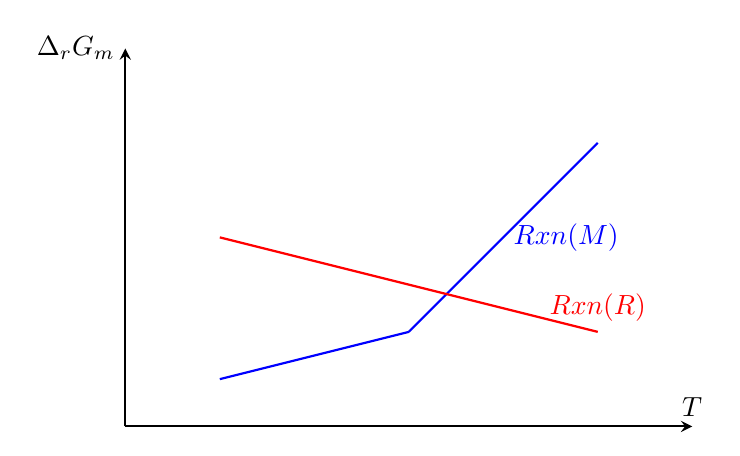
\begin{tikzpicture}[scale=1.2,
                    >=stealth,
                    axis/.style={thick,black}]

\draw[axis,->] (0,0) -- (6,0) node[above] {$T$}; 
\draw[axis,->] (0,0) -- (0,4) node[left] {$\Delta_r G_m$}; 

\draw[thick,blue] (1,0.5) -- (3,1) node[midway,above right]{};
\draw[thick,blue] (3,1) -- (5,3) node[midway,right] {$Rxn(\text{M})$};
\draw[thick,red] (1,2) -- (5,1) node[right,above] {$Rxn(\text{R})$};

\end{tikzpicture} 
\end{center}

The slope of each line is $-\Delta_r S_m$, and the temperature at which $\Delta_r G_m = 0$ is $T_0 = {\Delta_r H_m}/{\Delta_r S_m}$, the transition temperature above which the reaction becomes spontaneous. For coupled metal reduction reactions, a reducing agent can reduce a metal oxide if its line lies below the metal oxide line on the diagram.

A notable feature of the diagram is the kinks in the metal oxide lines, which arise from phase changes (melting or boiling) of the metal or its oxide, which change the entropy of the reaction and thus the slope of the line.
\end{definition}

\newpage
